% answers.tex —— 2002 年·上海卷·文科 · 参考答案与详细解析片段
% 由 tools/generate_projects.py 依来源总账自 2002/2002_数学真题_上海文_试题.md + 2002/2002_数学真题_上海文_解析正文.md + 2002/2002_数学真题_上海文_答案要点.md 生成，勿手改（改源 MD 后重跑）


\begin{gktip}
固定源 PDF 为印刷页码 110–111 的两页题面，不附答案。以下解析均依据题面独立复算；第 13、15、16、17 题图形在 LaTeX 工程中以 TikZ/PGFPlots 矢量源重绘。
\end{gktip}

\gkpart{一、填空题}

\begin{answer}
\gksolhead{1}{}

\textbf{题目}：

若 $z\in\mathbb C$，$(3+z)i=1$（$i$ 为虚数单位），则 $z=$\gkblank{}。

\Needspace{4\baselineskip}
\textbf{解析}

由 $(3+z)i=1$ 得 $3+z=1/i=-i$，所以 $z=-3-i$。

\gkanswer{答案：$-3-i$。}

\end{answer}
\begin{answer}
\gksolhead{2}{}

\textbf{题目}：

\Needspace{5\baselineskip}
已知向量 $\vec a$ 和 $\vec b$ 的夹角为 $120^\circ$，且 $|\vec a|=2$，$|\vec b|=5$，则

\nopagebreak[4]
\[
(2\vec a-\vec b)\cdot\vec a=
\]

\gkblank{}。

\Needspace{4\baselineskip}
\textbf{解析}

\nopagebreak[4]
\[
(2\vec a-\vec b)\cdot\vec a
=2|\vec a|^2-\vec a\cdot\vec b
=8-2\cdot5\cos120^\circ
=13.
\]

\gkanswer{答案：$13$。}

\end{answer}
\begin{answer}
\gksolhead{3}{}

\textbf{题目}：

\Needspace{5\baselineskip}
方程

\nopagebreak[4]
\[
\log_3(1-2\cdot3^x)=2x+1
\]

的解 $x=$\gkblank{}。

\Needspace{4\baselineskip}
\textbf{解析}

\Needspace{5\baselineskip}
令 $t=3^x>0$，则方程化为

\nopagebreak[4]
\[
\log_3(1-2t)=\log_3t^2
\Longrightarrow
1-2t=t^2.
\]

取正根 $t=\sqrt2-1$，故 $x=\log_3(\sqrt2-1)$。

\gkanswer{答案：$\log_3(\sqrt2-1)$。}

\end{answer}
\begin{answer}
\gksolhead{4}{}

\textbf{题目}：

若正四棱锥的底面边长为 $2\sqrt3\text{ cm}$，体积为 $4\text{ cm}^3$，则它的侧面与底面所成的二面角的大小是\gkblank{}。

\Needspace{4\baselineskip}
\textbf{解析}

\Needspace{5\baselineskip}
底面积为 $12$，由 $\frac13\cdot12h=4$ 得高 $h=1$。正四棱锥侧面与底面的二面角在过边中点的截面内满足

\nopagebreak[4]
\[
\tan\theta=\frac{h}{\sqrt3}=\frac1{\sqrt3},
\]

所以 $\theta=\pi/6$。

\gkanswer{答案：$\dfrac\pi6$。}

\end{answer}
\begin{answer}
\gksolhead{5}{}

\textbf{题目}：

\Needspace{5\baselineskip}
在二项式 $(1+3x)^n$ 和 $(2x+5)^n$ 的展开式中，各项系数之和分别记为 $a_n\text{、}b_n$，$n$ 是正整数，则

\nopagebreak[4]
\[
\lim_{n\to\infty}\frac{a_n-2b_n}{3a_n-4b_n}
\]

等于\gkblank{}。

\Needspace{4\baselineskip}
\textbf{解析}

\Needspace{5\baselineskip}
各项系数和分别为 $a_n=4^n$、$b_n=7^n$，故

\nopagebreak[4]
\[
\lim_{n\to\infty}\frac{4^n-2\cdot7^n}{3\cdot4^n-4\cdot7^n}
=\frac12.
\]

\gkanswer{答案：$\dfrac12$。}

\end{answer}
\begin{answer}
\gksolhead{6}{}

\textbf{题目}：

\Needspace{5\baselineskip}
已知圆

\nopagebreak[4]
\[
x^2+(y-1)^2=1
\]

和圆外一点 $P(-2,0)$，过点 $P$ 作圆的切线，则两条切线夹角的正切值是\gkblank{}。

\Needspace{4\baselineskip}
\textbf{解析}

\Needspace{5\baselineskip}
圆心为 $(0,1)$，半径为 $1$，$OP=\sqrt5$。若两切线夹角为 $\varphi$，则 $\sin(\varphi/2)=1/\sqrt5$，从而 $\tan(\varphi/2)=1/2$，故

\nopagebreak[4]
\[
\tan\varphi=\frac{2(1/2)}{1-(1/2)^2}=\frac43.
\]

\gkanswer{答案：$\dfrac43$。}

\end{answer}
\begin{answer}
\gksolhead{7}{}

\textbf{题目}：

在某次花样滑冰比赛中，发生裁判受贿事件，竞赛委员会决定将裁判由原来的 9 名增至 14 名，但只任取其中 7 名裁判的评分作为有效分。若 14 名裁判中有 2 人受贿，则有效分中没有受贿裁判的评分的概率是\gkblank{}。（结果用数值表示）

\Needspace{4\baselineskip}
\textbf{解析}

\Needspace{5\baselineskip}
有效评分中没有受贿裁判的概率为

\nopagebreak[4]
\[
\frac{\binom{12}{7}}{\binom{14}{7}}=\frac3{13}.
\]

\gkanswer{答案：$\dfrac3{13}$。}

\end{answer}
\begin{answer}
\gksolhead{8}{}

\textbf{题目}：

\Needspace{5\baselineskip}
抛物线

\nopagebreak[4]
\[
(y-1)^2=4(x-1)
\]

的焦点坐标是\gkblank{}。

\Needspace{4\baselineskip}
\textbf{解析}

$(y-1)^2=4(x-1)$ 的顶点为 $(1,1)$，其中 $p=2$，焦点为 $(1+p,1)=(2,1)$。

\gkanswer{答案：$(2,1)$。}

\end{answer}
\begin{answer}
\gksolhead{9}{}

\textbf{题目}：

某工程由下列工序组成，则工程总时数为\gkblank{}天。

\begin{center}
\begin{tabular}{lrrrrrr}
\toprule
工序 & $a$ & $b$ & $c$ & $d$ & $e$ & $f$ \\
\midrule
紧前工序 & — & — & $a\text{、}b$ & $c$ & $c$ & $d\text{、}e$ \\
工时数（天） & 2 & 3 & 2 & 5 & 4 & 1 \\
\bottomrule
\end{tabular}
\end{center}

\Needspace{4\baselineskip}
\textbf{解析}

\Needspace{5\baselineskip}
工序完成时间由关键路径决定。各路径中

\nopagebreak[4]
\[
b\to c\to d\to f:3+2+5+1=11
\]

最长，所以总工期为 11 天。

\gkanswer{答案：$11$ 天。}

\end{answer}
\begin{answer}
\gksolhead{10}{}

\textbf{题目}：

设函数 $f(x)=\sin2x$，若 $f(x+t)$ 是偶函数，则 $t$ 的一个可能值是\gkblank{}。

\Needspace{4\baselineskip}
\textbf{解析}

\nopagebreak[4]
\[
\sin(2x+2t)=\sin2x\cos2t+\cos2x\sin2t.
\]

要成为偶函数，须 $\cos2t=0$，可取 $t=\pi/4$。

\gkanswer{答案：$\dfrac\pi4$。}

\end{answer}
\begin{answer}
\gksolhead{11}{}

\textbf{题目}：

\Needspace{5\baselineskip}
若数列 $\{a_n\}$ 中，$a_1=3$，且 $a_{n+1}=a_n^2$（$n$ 是正整数），则数列的通项

\nopagebreak[4]
\[
a_n=
\]

\gkblank{}。

\Needspace{4\baselineskip}
\textbf{解析}

\Needspace{5\baselineskip}
递推取对数或直接迭代得

\nopagebreak[4]
\[
a_1=3,\quad a_2=3^2,\quad a_3=3^4,\quad
a_n=3^{2^{n-1}}.
\]

\gkanswer{答案：$a_n=3^{2^{n-1}}$。}

\end{answer}
\begin{answer}
\gksolhead{12}{}

\textbf{题目}：

已知函数 $y=f(x)$（定义域为 $D$，值域为 $A$）有反函数 $y=f^{-1}(x)$，则方程 $f(x)=0$ 有解 $x=a$，且 $f(x)>x$（$x\in D$）的充要条件是 $y=f^{-1}(x)$ 满足\gkblank{}。

\Needspace{4\baselineskip}
\textbf{解析}

\Needspace{5\baselineskip}
由 $f(a)=0$ 得 $f^{-1}(0)=a$。又 $f(x)>x$ 对 $x\in D$ 成立，令 $y=f(x)$，则对 $y\in A$ 有 $f^{-1}(y)<y$。两条件合起来即

\nopagebreak[4]
\[
f^{-1}(0)=a,\qquad f^{-1}(x)<x\quad(x\in A).
\]

\gkanswer{答案：$f^{-1}(0)=a$ 且 $f^{-1}(x)<x$（$x\in A$）。}

\end{answer}
\gkpart{二、选择题}

\begin{answer}
\gksolhead{13}{}

\textbf{题目}：

如图，与复平面中的阴影部分（含边界）对应的复数集合是\mbox{（　　）}
\nopagebreak[4]
\begin{center}% 2002 年上海文科第 13 题：复平面阴影区域
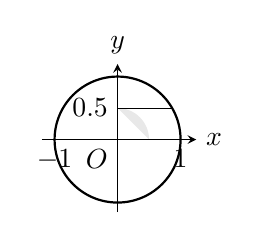
\begin{tikzpicture}[scale=0.8, >=stealth]
  \fill[gray!18] (0,0.5) arc (90:0:0.5) -- (0,0.5) -- cycle;
  \draw[thick] (0,0) circle (1);
  \draw[->] (-1.2,0)--(1.25,0) node[right] {$x$};
  \draw[->] (0,-1.15)--(0,1.2) node[above] {$y$};
  \draw (0,0.5)--(0.866,0.5);
  \node[left] at (0,0.5) {$0.5$};
  \node[below left] at (0,0) {$O$};
  \node[below] at (-1,0) {$-1$};
  \node[below] at (1,0) {$1$};
\end{tikzpicture}
\end{center}
\nopagebreak[4]
（A）$\{z\mid |z|=1,\ \operatorname{Re}z\ge\dfrac12,\ z\in\mathbb C\}$

（B）$\{z\mid |z|\le1,\ \operatorname{Re}z\ge\dfrac12,\ z\in\mathbb C\}$

（C）$\{z\mid |z|=1,\ \operatorname{Im}z\ge\dfrac12,\ z\in\mathbb C\}$

（D）$\{z\mid |z|\le1,\ \operatorname{Im}z\ge\dfrac12,\ z\in\mathbb C\}$

\Needspace{4\baselineskip}
\textbf{解析}

图中阴影是单位圆内、直线 $y=1/2$ 上方的圆弓形区域，所以满足 $|z|\le1$ 且 $\operatorname{Im}z\ge1/2$，选 D。

\gkanswer{答案：D。}

\end{answer}
\begin{answer}
\gksolhead{14}{}

\textbf{题目}：

已知直线 $l\text{、}m$，平面 $\alpha\text{、}\beta$，且 $l\perp\alpha$，$m\subset\beta$，给出下列四个命题：

① 若 $\alpha\parallel\beta$，$l\perp m$；② $l\perp m$，$\alpha\parallel\beta$；③ 若 $\alpha\perp\beta$，则 $l\parallel m$；④ 若 $l\parallel m$，$\alpha\perp\beta$。

其中正确命题的个数是\mbox{（　　）}

（A）1 个　　（B）2 个　　（C）3 个　　（D）4 个

\Needspace{4\baselineskip}
\textbf{解析}

在 $l\perp\alpha$、$m\subset\beta$ 的条件下，①和④成立，②、③不能由题设推出，故正确命题有 2 个，选 B。

\gkanswer{答案：B。}

\end{answer}
\begin{answer}
\gksolhead{15}{}

\textbf{题目}：

函数 $y=x+\sin|x|$，$x\in[-\pi,\pi]$ 的大致图象是\mbox{（　　）}
\nopagebreak[4]
\begin{center}% 2002 年上海文科第 15 题：函数图象选项示意
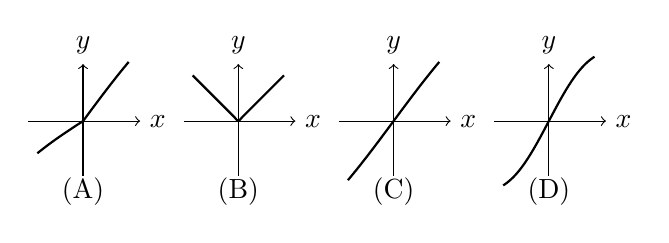
\begin{tikzpicture}[scale=0.58]
  \foreach \shift/\lab in {0/A,3.4/B,6.8/C,10.2/D} {
    \begin{scope}[xshift=\shift cm]
      \draw[->] (-1.2,0)--(1.25,0) node[right] {$x$};
      \draw[->] (0,-1.2)--(0,1.25) node[above] {$y$};
      \node at (0,-1.55) {(\lab)};
    \end{scope}
  }
  \draw[thick, domain=-1:1, smooth] plot ({\x},{\x+0.35*sin(deg(abs(\x)))});
  \draw[thick, domain=-1:1, smooth, xshift=3.4cm] plot ({\x},{abs(\x)});
  \draw[thick, domain=-1:1, smooth, xshift=6.8cm] plot ({\x},{\x+0.35*sin(deg(\x))});
  \draw[thick, domain=-1:1, smooth, xshift=10.2cm] plot ({\x},{\x+0.45*sin(deg(2*\x))});
\end{tikzpicture}
\end{center}
\nopagebreak[4]
（A）　　（B）　　（C）　　（D）

\Needspace{4\baselineskip}
\textbf{解析}

\nopagebreak[4]
\[
f(x)=x+\sin|x|=
\begin{cases}
x-\sin x,&x<0,\\
x+\sin x,&x\ge0.
\end{cases}
\]

函数整体递增，在原点左侧切线斜率趋于 0，右侧切线斜率为 2，且左右形状不关于原点对称。与图形比较选 A。

\gkanswer{答案：A。}

\end{answer}
\begin{answer}
\gksolhead{16}{}

\textbf{题目}：

一般地，家庭用电量（千瓦时）与气温（摄氏度）有一定的关系。图（1）表示某年 12 个月中每月的平均气温，图（2）表示某家庭在这年 12 个月中每月的用电量。根据这些信息，以下关于该家庭用电量与气温间关系的叙述中，正确的是\mbox{（　　）}
\nopagebreak[4]
\begin{center}% 2002 年上海文科第 16 题：月度气温与用电量统计图
\begin{tikzpicture}[x=0.34cm,y=0.035cm]
  \draw[->] (0,0)--(13,0) node[right] {月份};
  \draw[->] (0,0)--(0,32) node[above] {气温};
  \foreach \x/\h in {1/3,2/8,3/14,4/18,5/23,6/27,7/28,8/24,9/17,10/12,11/5,12/2}
    \draw[fill=gray!15] (\x-0.42,0) rectangle (\x+0.42,\h);
  \begin{scope}[xshift=6cm,yshift=0cm]
    \draw[->] (0,0)--(13,0) node[right] {月份};
    \draw[->] (0,0)--(0,130) node[above] {用电量};
    \foreach \x/\h in {1/115,2/120,3/95,4/80,5/75,6/80,7/110,8/120,9/95,10/75,11/85,12/100}
      \draw[fill=gray!15] (\x-0.42,0) rectangle (\x+0.42,\h);
  \end{scope}
\end{tikzpicture}
\end{center}
\nopagebreak[4]
（A）气温最高时，用电量最多

（B）气温最低时，用电量最少

（C）当气温大于某一值时，用电量随气温增高而增加

（D）当气温小于某一值时，用电量随气温降低而增加

\Needspace{4\baselineskip}
\textbf{解析}

用电量在冬季低温时较高，在夏季高温时也较高，因此不能断言最高温对应最高用电量，也不能断言最低温对应最低用电量；合理的描述是气温低于某值时，降温会使取暖用电增加，选 D。

\gkanswer{答案：D。}

\end{answer}
\gkpart{三、解答题}

\begin{answer}
\gksolhead{17}{}

\textbf{题目}：

如图，在直三棱柱 $ABO-A'B'O'$ 中，$OO'=4$，$OA=4$，$OB=3$，$\angle AOB=90^\circ$，$D$ 是线段 $A'B'$ 的中点，$P$ 是侧棱 $BB'$ 上的一点。若 $OP\perp BD$，求 $OP$ 与底面 $AOB$ 所成角的大小。（结果用反三角函数值表示）
\nopagebreak[4]
\begin{center}% 2002 年上海文科第 17 题：直三棱柱空间图
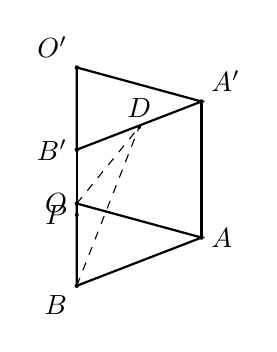
\begin{tikzpicture}[>=stealth, scale=0.72]
  \coordinate (O) at (0,0);
  \coordinate (A) at (2.2,-0.6);
  \coordinate (B) at (0,-1.45);
  \coordinate (Op) at (0,2.4);
  \coordinate (Ap) at (2.2,1.8);
  \coordinate (Bp) at (0,0.95);
  \coordinate (D) at (1.1,1.35);
  \coordinate (P) at (0,-0.2);
  \draw[thick] (O)--(A)--(B)--cycle;
  \draw[thick] (Op)--(Ap)--(Bp)--cycle;
  \draw[thick] (O)--(Op) (A)--(Ap) (B)--(Bp);
  \draw[dashed] (O)--(D) (B)--(D);
  \draw[thick] (O)--(P);
  \fill (O) circle (1.1pt) node[left] {$O$};
  \fill (A) circle (1.1pt) node[right] {$A$};
  \fill (B) circle (1.1pt) node[below left] {$B$};
  \fill (Op) circle (1.1pt) node[above left] {$O'$};
  \fill (Ap) circle (1.1pt) node[above right] {$A'$};
  \fill (Bp) circle (1.1pt) node[left] {$B'$};
  \fill (D) circle (1.0pt) node[above] {$D$};
  \fill (P) circle (1.0pt) node[left] {$P$};
\end{tikzpicture}
\end{center}
\nopagebreak[4]
\Needspace{4\baselineskip}
\textbf{解析}

\Needspace{5\baselineskip}
取 $O=(0,0,0)$、$A=(4,0,0)$、$B=(0,3,0)$，并令 $O'=(0,0,4)$、$A'=(4,0,4)$、$B'=(0,3,4)$。则

\nopagebreak[4]
\[
D=(2,\tfrac32,4),\qquad P=(0,3,p).
\]

\Needspace{5\baselineskip}
由 $OP\perp BD$，

\nopagebreak[4]
\[
(0,3,p)\cdot(2,-\tfrac32,4)=0
\Longrightarrow p=\frac98.
\]

\Needspace{5\baselineskip}
直线 $OP$ 在底面上的投影长度为 $OB=3$，所以所成角 $\theta$ 满足

\nopagebreak[4]
\[
\tan\theta=\frac{OP\text{ \text{的竖直分量}}}{OP\text{ \text{的水平投影}}}=\frac{9/8}{3}=\frac38.
\]

\gkanswer{答案：$\arctan\dfrac38$。}

\end{answer}
\begin{answer}
\gksolhead{18}{}

\textbf{题目}：

已知点 $A(-\sqrt3,0)$ 和 $B(\sqrt3,0)$，动点 $C$ 到 $A\text{、}B$ 两点的距离之差的绝对值为 2，点 $C$ 的轨迹与直线 $y=x-2$ 交于 $D\text{、}E$ 两点，求线段 $DE$ 的长。

\Needspace{4\baselineskip}
\textbf{解析}

\Needspace{5\baselineskip}
轨迹是焦点为 $A\text{、}B$、实轴长为 $2$ 的双曲线

\nopagebreak[4]
\[
x^2-\frac{y^2}{2}=1.
\]

\Needspace{5\baselineskip}
代入直线 $y=x-2$：

\nopagebreak[4]
\[
x^2-\frac{(x-2)^2}{2}=1
\Longrightarrow x^2+4x-6=0.
\]

\Needspace{5\baselineskip}
两交点横坐标之差为 $2\sqrt{10}$，直线斜率为 1，故

\nopagebreak[4]
\[
DE=\sqrt{1^2+1^2}\cdot2\sqrt{10}=4\sqrt5.
\]

\gkanswer{答案：$4\sqrt5$。}

\end{answer}
\begin{answer}
\gksolhead{19}{}

\textbf{题目}：

\Needspace{5\baselineskip}
已知函数

\nopagebreak[4]
\[
f(x)=x^2+2ax+2,\qquad x\in[-5,5].
\]

（1） 当 $a=-1$ 时，求函数 $f(x)$ 的最大值与最小值。

（2） 求实数 $a$ 的取值范围，使 $y=f(x)$ 在区间 $[-5,5]$ 上是单调函数。

\Needspace{4\baselineskip}
\textbf{解析}

\gksubpart{(1)}

当 $a=-1$ 时，$f(x)=(x-1)^2+1$，故最小值为 $1$；端点值中 $f(-5)=37$ 最大。

\gksubpart{(2)}

$f'(x)=2x+2a$。若在整个区间上递增，需 $f'(-5)\ge0$，即 $a\ge5$；若在整个区间上递减，需 $f'(5)\le0$，即 $a\le-5$。

\gkanswer{答案（1）：最大值 $37$，最小值 $1$。}

\gkanswer{答案（2）：$a\le-5$ 或 $a\ge5$。}

\end{answer}
\begin{answer}
\gksolhead{20}{}

\textbf{题目}：

某商场在促销期间规定：商场内所有商品按标价的 80\% 出售，同时，当顾客在该商场内消费满一定金额后，按如下方案获得相应金额的奖券：

\begin{center}
\begin{tabular}{lrrrrr}
\toprule
消费金额的范围 & $[200,400)$ & $[400,500)$ & $[500,700)$ & $[700,900)$ & $\cdots$ \\
\midrule
获得奖券的金额 & 30 & 60 & 100 & 130 & $\cdots$ \\
\bottomrule
\end{tabular}
\end{center}

购买商品得到的优惠额为折扣额与奖券金额之和。设购买商品得到的优惠率为优惠额与商品标价之比，试问：

（1） 若购买一件标价为 1000 元的商品，顾客得到的优惠率是多少？

（2） 对于标价在 $[500,800]$ 元内的商品，顾客购买标价为多少元的商品，可得到不小于 $\dfrac13$ 的优惠率？

\Needspace{4\baselineskip}
\textbf{解析}

\gksubpart{(1)}

\Needspace{5\baselineskip}
标价 1000 元时消费金额为 800 元，奖券为 130 元，优惠额为

\nopagebreak[4]
\[
1000\times20\%+130=330,
\]

优惠率为 $33\%$。

\gksubpart{(2)}

\Needspace{5\baselineskip}
设标价为 $x$。当 $500\le x<625$ 时，奖券为 60 元，优惠率为 $0.2+60/x<1/3$；当 $625\le x\le800$ 时，奖券为 100 元，条件为

\nopagebreak[4]
\[
0.2+\frac{100}{x}\ge\frac13
\Longleftrightarrow x\le750.
\]

故 $x\in[625,750]$。

\gkanswer{答案（1）：$33\%$。}

\gkanswer{答案（2）：$625$ 元至 $750$ 元。}

\end{answer}
\begin{answer}
\gksolhead{21}{}

\textbf{题目}：

已知函数 $f(x)=a\cdot b^x$ 的图象过点 $A(4,\dfrac14)$ 和 $B(5,1)$。

（1） 求函数 $f(x)$ 的解析式；

（2） 记 $a_n=\log_2f(n)$，$n$ 是正整数，$S_n$ 是数列 $\{a_n\}$ 的前 $n$ 项和，解关于 $n$ 的不等式 $a_nS_n\le0$；

（3） 对于（2）中的 $a_n$ 与 $S_n$，整数 96 是否为数列 $\{a_nS_n\}$ 中的项？若是，则求出相应的项数；若不是，则说明理由。

\Needspace{4\baselineskip}
\textbf{解析}

\gksubpart{(1)}

\Needspace{5\baselineskip}
由两点条件

\nopagebreak[4]
\[
ab^4=\frac14,\qquad ab^5=1,
\]

得 $b=4$、$a=1/1024$，所以 $f(x)=2^{2x-10}$。

\gksubpart{(2)}

\Needspace{5\baselineskip}
于是

\nopagebreak[4]
\[
a_n=2n-10,\qquad
S_n=\sum_{k=1}^n(2k-10)=n(n-9).
\]

 $a_nS_n=2n(n-5)(n-9)\le0$，故正整数解为 $n=5,6,7,8,9$。

\gksubpart{(3)}

若 $a_nS_n=104$，则 $n(n-5)(n-9)=52$。逐段考察正整数区间可知无整数解，因此 104 不是该数列的项。

\gkanswer{答案（1）：$f(x)=2^{2x-10}$。}

\gkanswer{答案（2）：$n=5,6,7,8,9$。}

\gkanswer{答案（3）：不是。}

\end{answer}
\begin{answer}
\gksolhead{22}{}

\textbf{题目}：

\Needspace{5\baselineskip}
规定

\nopagebreak[4]
\[
C_x^m=\frac{x(x-1)\cdots(x-m+1)}{m!},
\]

其中 $x\in\mathbb R$，$m$ 是正整数，且 $C_0^x=1$。这是组合数 $C_n^m$（$n\text{、}m$ 是正整数，且 $m\le n$）的一种推广。

（1） 求 $C_{-15}^3$ 的值；

（2） 设 $x>0$，当 $x$ 为何值时，$\dfrac{C_x^3}{(C_x^1)^2}$ 取得最小值？

（3） 组合数的两个性质：① $C_n^m=C_n^{n-m}$；② $C_n^m+C_n^{m-1}=C_{n+1}^m$ 是否都能推广到 $C_x^m$（$x\in\mathbb R$，$m$ 是正整数）的情形？若能推广，则写出推广的形式并给出证明；若不能，则说明理由。

\Needspace{4\baselineskip}
\textbf{解析}

\gksubpart{(1)}

\nopagebreak[4]
\[
C_{-15}^3=\frac{(-15)(-16)(-17)}6=-680.
\]

\gksubpart{(2)}

\nopagebreak[4]
\[
\frac{C_x^3}{(C_x^1)^2}
=\frac{x(x-1)(x-2)/6}{x^2}
=\frac16\left(x+\frac2x-3\right).
\]

由 $x+2/x\ge2\sqrt2$，最小值在 $x=\sqrt2$ 时取得。

\gksubpart{(3)}

\Needspace{5\baselineskip}
性质①不能对任意实数推广，因为右端下标 $x-m$ 不一定是正整数，且原定义只允许下标为正整数。性质②可由乘积展开直接验证：

\nopagebreak[4]
\[
C_x^m+C_x^{m-1}=C_{x+1}^m.
\]

\gkanswer{答案（1）：$-680$。}

\gkanswer{答案（2）：$x=\sqrt2$。}

\gkanswer{答案（3）：性质①不能对任意实数 $x$ 推广；性质②可推广为 $C_x^m+C_x^{m-1}=C_{x+1}^m$。}

\end{answer}